\documentclass{homework}

\title{Simulation 2}
\author{Kevin Evans}
\studentid{11571810}
\date{March 13, 2020}
\setclass{EE}{311}
\usepackage{amssymb}
\usepackage{mathtools}

\usepackage{amsthm}
\usepackage{amsmath}
\usepackage{slashed}
\usepackage{relsize}
\usepackage{threeparttable}
\usepackage{float}
\usepackage{booktabs}
\usepackage{boldline}
\usepackage{changepage}
\usepackage{physics}
\usepackage[inter-unit-product =\cdot]{siunitx}
\usepackage{setspace}

\usepackage[makeroom]{cancel}
\usepackage{pgfplots}

\usepackage{multicol}
\usepackage{tcolorbox}
\usepackage{enumitem}
\usepackage{times}
\usepackage{mhchem}
\usepackage{graphicx}

\DeclareSIUnit{\year}{yr}
\begin{document}
	\maketitle
	
	\subsubsection*{(a) Circuit in Virtuoso}
	\begin{minipage}[t]{0.5\linewidth}
		\centering NMOS
		
		\noindent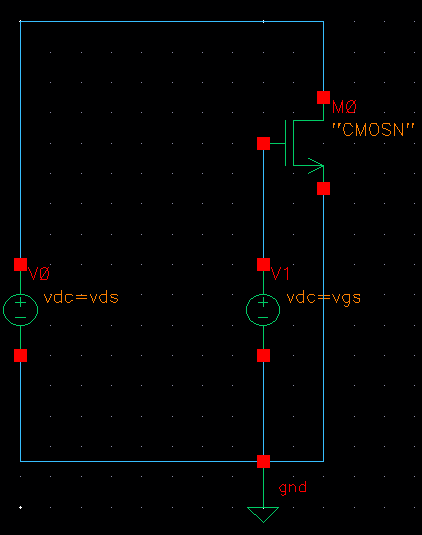
\includegraphics[width=1\linewidth]{hw2}
	\end{minipage}
	\begin{minipage}[t]{0.5\linewidth}
	\centering PMOS
	
	\noindent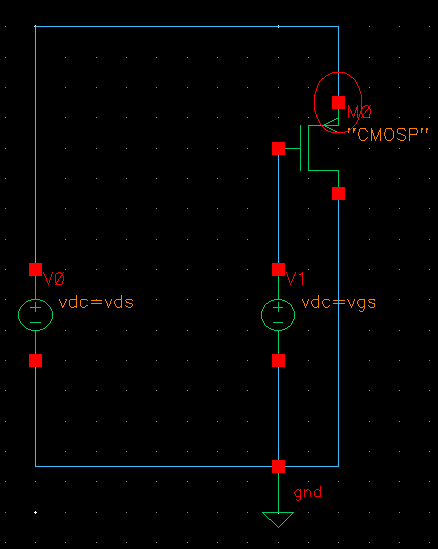
\includegraphics[width=1\linewidth]{hw2pmos}
	
	\raggedright
	Was I supposed to sweep $V_{gs}$ through negative voltages or flip the polarity of the dc supply? The instructions didn't mention it and I thought that was a little strange...
	\end{minipage}
	\pagebreak
	\subsubsection*{(b) NMOS $I$-$V_{ds}$}	
	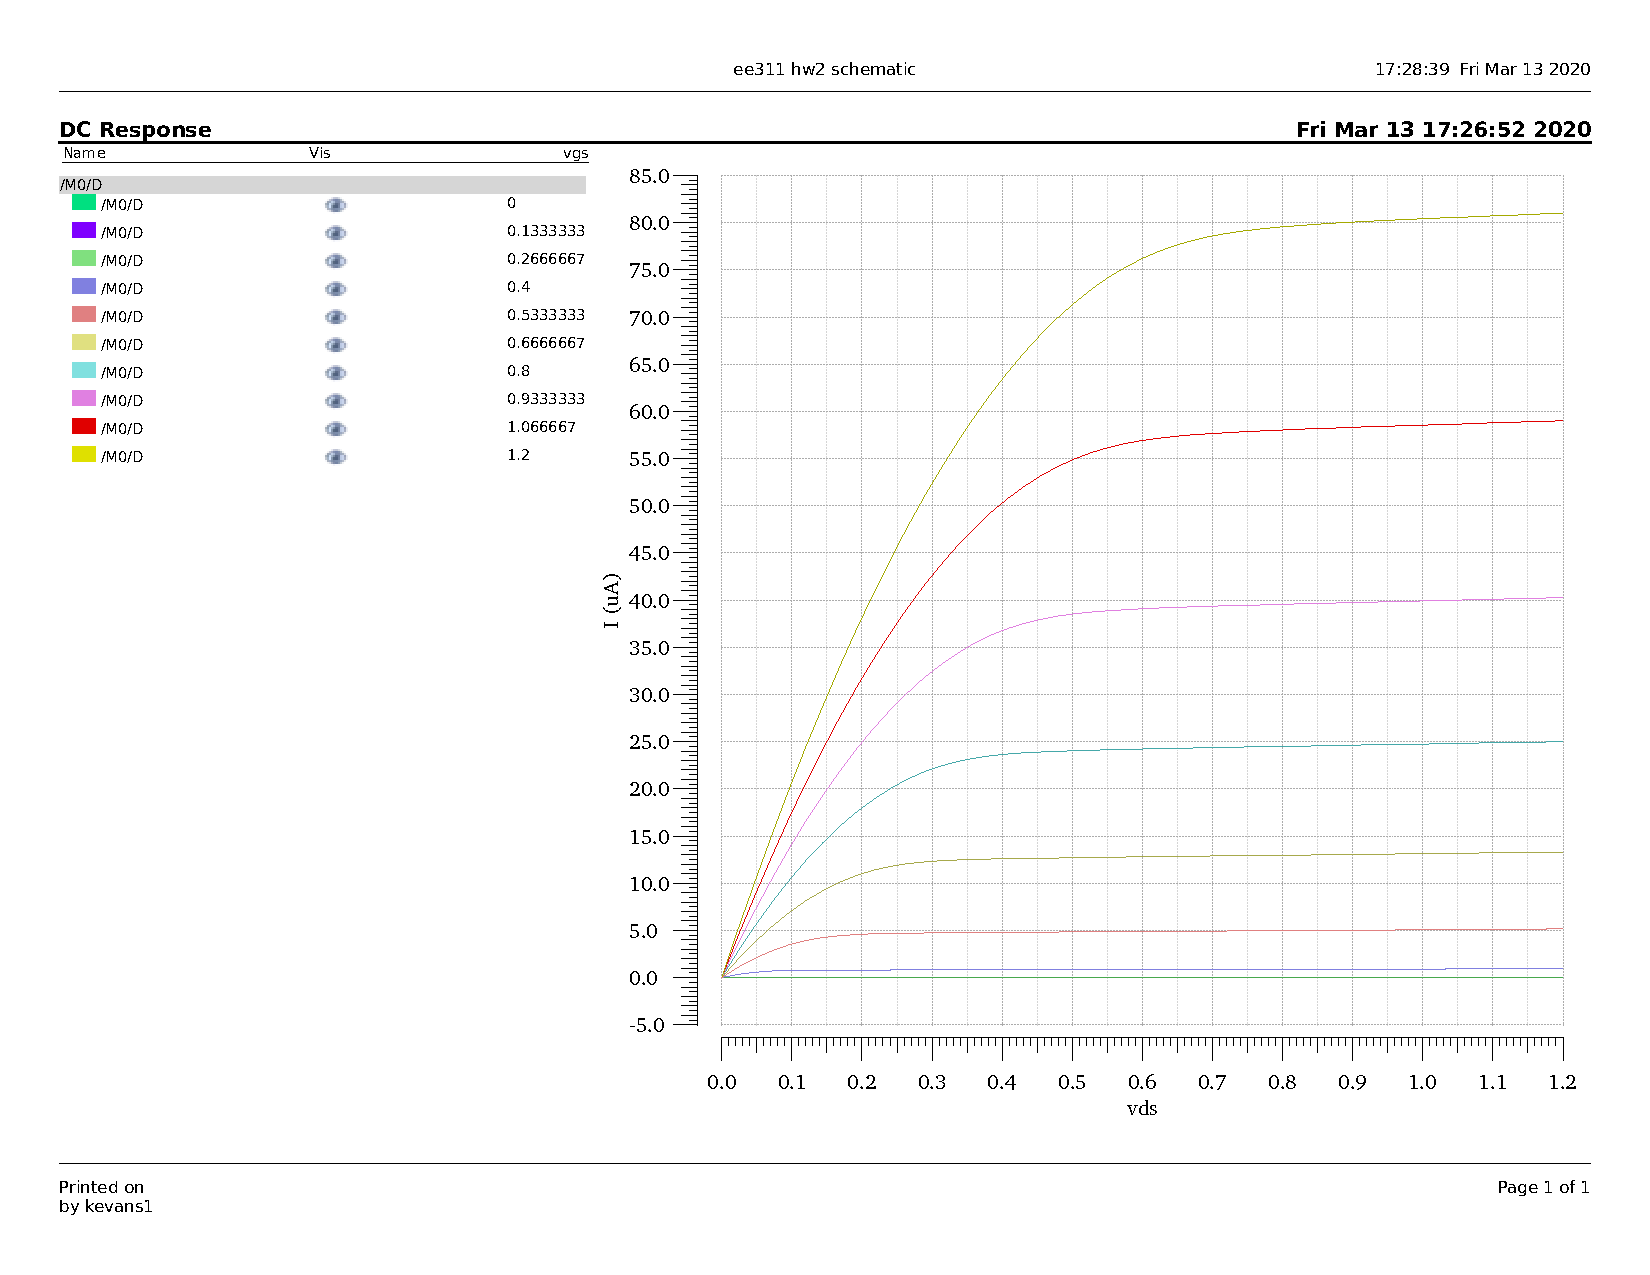
\includegraphics[width=1\linewidth]{nmos}
	
	\pagebreak
	\subsubsection*{(c) PMOS $I$-$V_{ds}$}			
	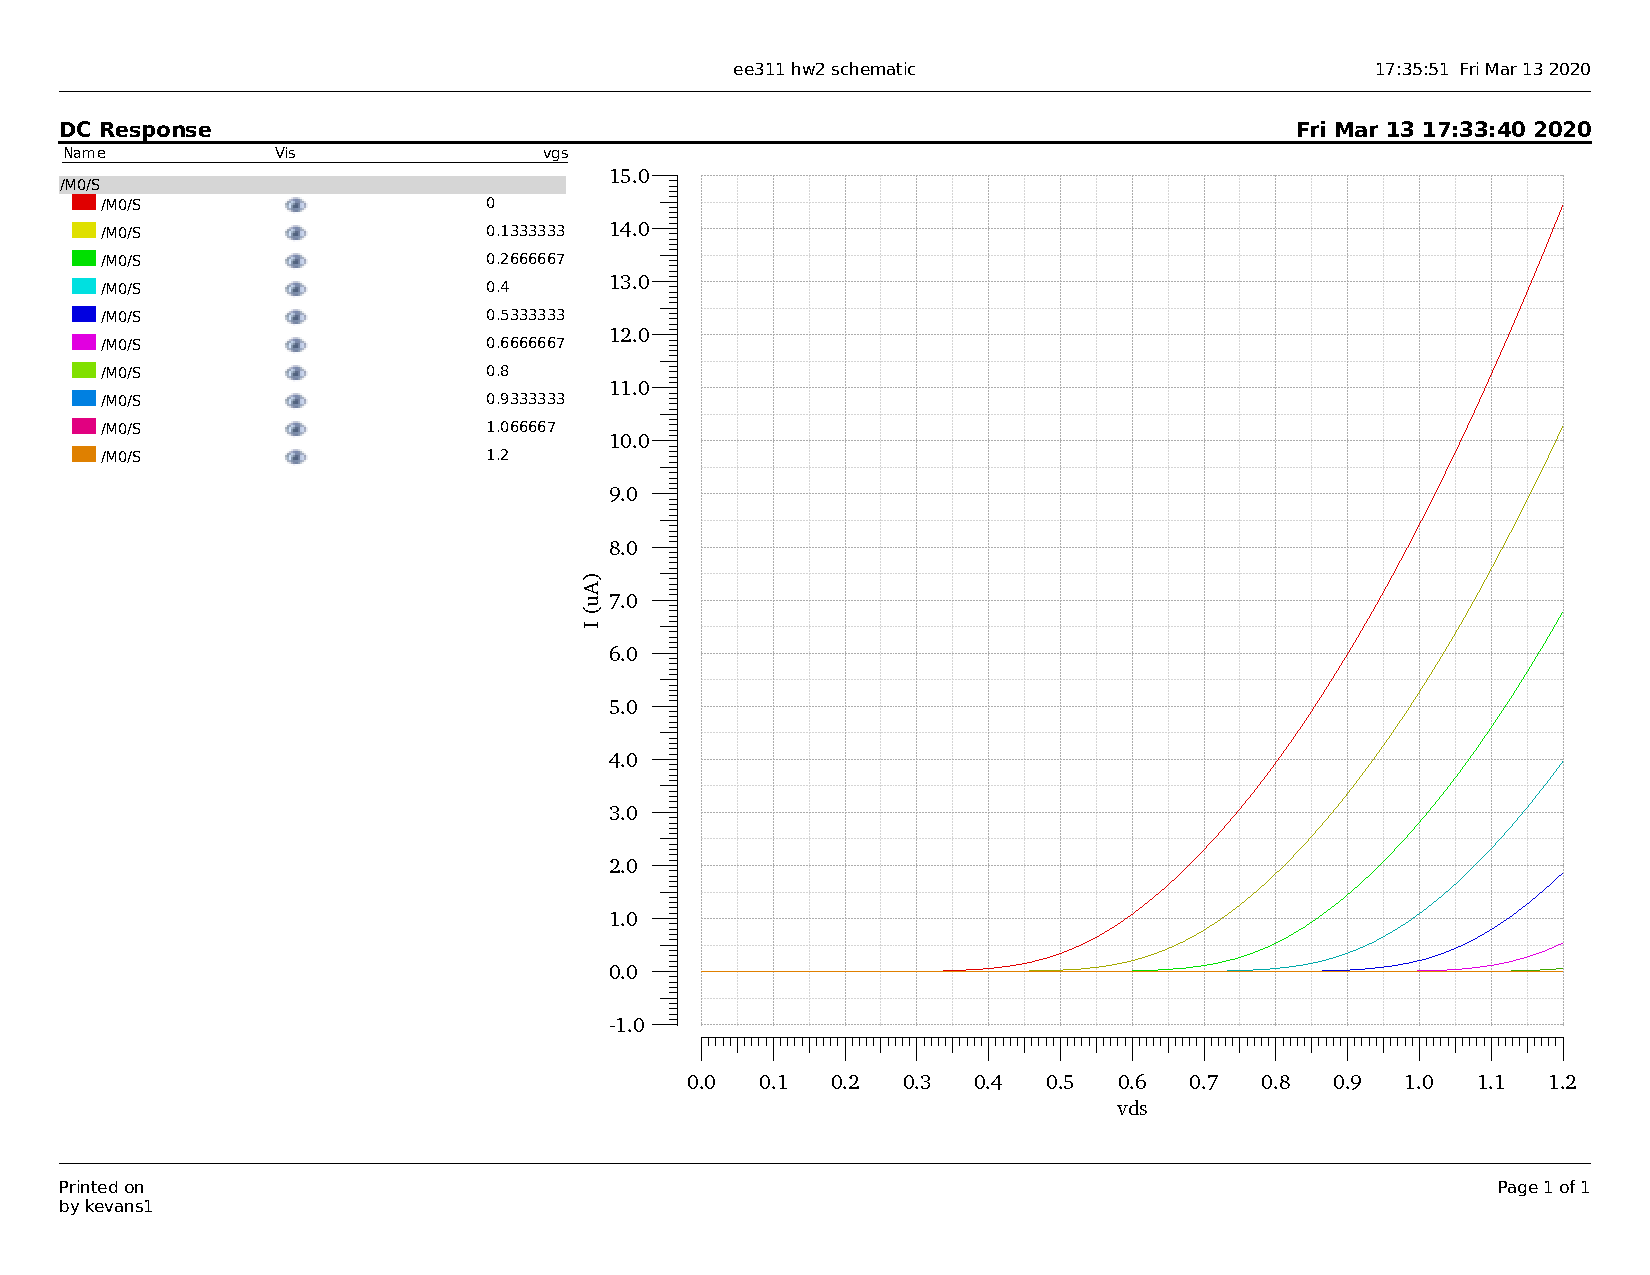
\includegraphics[width=1\linewidth]{pmos}

	\pagebreak
	\subsubsection*{(d) Discussion}
	\begin{enumerate}
		\item[i.] The NMOS operates in the cutoff--triode--saturation region as $V_{ds}$ increases. Current runs from the top terminal (drain) to the lower (bottom). The PMOS operates in the cutoff--saturation region as $V_{ds}$ increases and is operating ``flipped'', as the current is running from the lower terminal up to the top. As the PMOS is acting in reverse, the current plots are flipped.
		
		\item[ii.] The NMOS curve family experiences all three regions: \begin{itemize}
			\item The lower $V_{gs}$ curves are in the cutoff region, where $V_{GS} < \SI{0.4}{\V}$. The threshold voltage $V_{tn}$ is around \num{0.267} to \SI{0.4}{\V}.
			\item For the upper curves ($V_{gs} \ge 0.4$), the left-side is in the triode region, the right-side is in the saturation region.
			\item For example: the orange curve ($V_{gs} = 1.2$), it is in the triode region from $V_{DS} \approx 0$ to $0.7$. After $0.7$, it is in the saturation region.
		\end{itemize}
	
		For the PMOS: 
		
		\begin{itemize}
			\item All the plots are in the cutoff region until current begins to flow. For $V_{gs} > 0.5$ or so, the transistors barely exit from the cutoff region.
			\item It only operates at saturation afterwards, as the drain-source terminals are flipped in this situation. 
		\end{itemize}
		
		\item[iii.] The plots are the showing the expected current behavior. For the NMOS, the curves go through the cutoff--triode--saturation regions. The PMOS goes from the cutoff to the saturation as the transistor as the threshold voltage is negative and the drain-source voltage is negative as well.
		
		\item[iv.] If you double the transistor width, the $k_n$ and $k_p$ values are doubled, so the current through the drain/source will double as $i_D \propto k \propto W$. As an example, if you have an NMOS in both the triode/saturation region (red dashed line) and double the width, you would expect the current to double (blue solid line):
		\begin{center}
			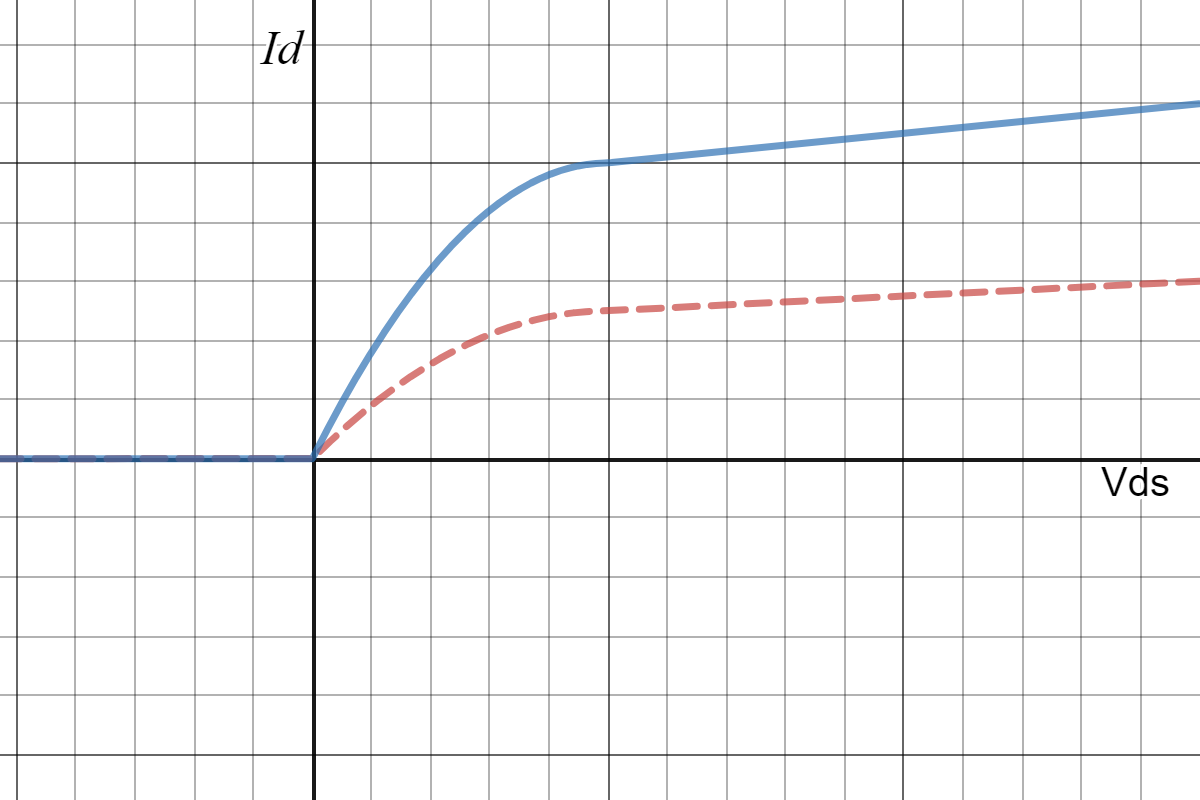
\includegraphics[width=0.8\linewidth]{plot}
		\end{center}
		
	\end{enumerate}
\end{document}